%%%%%%%%%%%%%%%%%%%%%%%%%%%%%%%%%%%%%%%%%%%%%%%%%%%%%%%%%%%%%%%%%%%%%%
% LaTeX Example: Project Report
%
% Source: http://www.howtotex.com
%
% Feel free to distribute this example, but please keep the referral
% to howtotex.com
% Date: March 2011 
% 
%%%%%%%%%%%%%%%%%%%%%%%%%%%%%%%%%%%%%%%%%%%%%%%%%%%%%%%%%%%%%%%%%%%%%%
% How to use writeLaTeX: 
%
% You edit the source code here on the left, and the preview on the
% right shows you the result within a few seconds.
%
% Bookmark this page and share the URL with your co-authors. They can
% edit at the same time!
%
% You can upload figures, bibliographies, custom classes and
% styles using the files menu.
%
% If you're new to LaTeX, the wikibook is a great place to start:
% http://en.wikibooks.org/wiki/LaTeX
%
%%%%%%%%%%%%%%%%%%%%%%%%%%%%%%%%%%%%%%%%%%%%%%%%%%%%%%%%%%%%%%%%%%%%%%
% Edit the title below to update the display in My Documents
%\title{Project Report}
%
%%% Preamble
\documentclass[paper=a4, fontsize=11pt, margin=1in]{scrartcl}
\usepackage[T1]{fontenc}
\usepackage{fourier}
\usepackage{longtable}
\usepackage[english]{babel}															% English language/hyphenation
\usepackage[protrusion=true,expansion=true]{microtype}	
\usepackage{amsmath,amsfonts,amsthm} % Math packages
\usepackage[pdftex]{graphicx}	
\usepackage{url}
\usepackage[colorlinks=true]{hyperref}
\usepackage{multicol}
\setlength{\footskip}{120pt}
\usepackage{caption} 
\usepackage{subcaption}

%%% Custom sectioning
\usepackage{sectsty}
\allsectionsfont{\centering \normalfont\scshape}


%%% Custom headers/footers (fancyhdr package)
\usepackage{fancyhdr}
\pagestyle{fancyplain}
\fancyhead{}											% No page header
\fancyfoot[L]{}											% Empty 
\fancyfoot[C]{}											% Empty
\fancyfoot[C]{\thepage}									% Pagenumbering
\renewcommand{\headrulewidth}{0pt}			% Remove header underlines
\renewcommand{\footrulewidth}{0pt}				% Remove footer underlines
\setlength{\headheight}{12.6pt}


%%% Equation and float numbering
\numberwithin{equation}{section}		% Equationnumbering: section.eq#
\numberwithin{figure}{section}			% Figurenumbering: section.fig#
\numberwithin{table}{section}				% Tablenumbering: section.tab#

\setlength{\parindent}{0pt}
%%% Maketitle metadata
\newcommand{\horrule}[1]{\rule{\linewidth}{#1}} 	% Horizontal rule

\title{
		%\vspace{-1in} 	
		\usefont{OT1}{bch}{b}{n}
		\normalfont \normalsize \textsc{University of Maryland Science Academy} \\ [25pt]
		\horrule{0.5pt} \\[0.4cm]
		\huge A study in the effectiveness of various \\Deep Q-Network flavors  \\
		\horrule{2pt} \\[0.5cm]
}
\author{
		\normalfont 								\normalsize
        Sushant Karki\\[-3pt]		\normalsize
        \today
}
\date{}

\setlength{\parindent}{0pt}

%%% Begin document
\begin{document}
\maketitle
\section{\textbf{Abstract}}

On January 1, 2013, DeepMind published a paper called "Playing Atari with Deep Reinforcement Learning" introducing their algorithm called Deep Q-Network (DQN) which revolutionized the field of reinforcement learning. For the first time they had brought together Deep Learning and Q-learning and showed impressive results applying deep reinforcement learning to Atari games with their agents performing at or over human level expertise in almost all the games trained on.\\

A Deep Q-Network utilizes a deep neural network to estimate the q-values for each action, allowing the policy to select the action with the maximum q-values. This use of deep neural network to get q-values was immensely superior to implementing q-table look-ups and widened the applicability of q-learning to more complex reinforcement learning environments.\\

While revolutionary, the original version of DQN had a few problems, especially its slow/inefficient learning process. Over these past 9 years, a few improved versions of DQNs have become popular. This project is an attempt to study the effectiveness of a few of these DQN flavors, what problems they solve and compare their performance in the same reinforcement learning environment.


\pagebreak
\section{Deep Q-Networks and its flavors}


\begin{itemize}
\item \textbf{Vanilla DQN}\\\\
    The vanilla (original) DQN uses 2 neural networks: the \textbf{online} network and the \textbf{target} network. The online network is the main neural network that the agent uses to select the best action for a given state. The target neural network is usually a copy of the online network. It is used to get the "target" q-values for each action for a particular state. i.e. During the learning phase, since we don't have actual ground truths for future q-values, these q-values from the target network will be used as labels optimize the network. 

    The target network calculates the target q-values by using the following Bellman equation: 
    \begin{align}
	Q(s_t, a_t) = 
			r_{t+1} + \gamma \max _{a_{t+1} \in A} Q(s_{t+1}, a_{t+1}) 
    \end{align}
where, \\

\hspace*{10mm}$Q(s_t, a_t)$ \hspace{25}= \hspace{5} The target q-value (ground truth) for a past experience in the \hspace*{39mm}replay memory

\hspace*{10mm}$r_{t+1}$\hspace{46}= \hspace{5} The reward that was obtained for taking the chosen action in \hspace*{39mm}that particular experience

\hspace*{10mm}$\gamma$\hspace{60}= \hspace{5} The discount factor for future rewards

\hspace*{10mm}$Q(s_{t+1}, a_{t+1})$ \hspace{5}= \hspace{5} The q-value for best action (based on the policy) for the next \hspace*{39mm}state for that particular experience
    
    
    \item \textbf{Double DQN}\\\\
    One of the problems with vanilla DQN is the way it calculates its target values (ground-truth).
    We can see from the bellman equation above that the target network uses the \textbf{max} q-value directly in the equation. This is found to almost always overestimate the q-value because using the \textbf{max} function introduces the maximization-bias to our estimates. Using max will give the largest value even if that specific max value was an outlier, thus skewing our estimates.\\

    The Double DQN solves this problem by changing the original algorithm to the following:

    \begin{enumerate}
        \item Instead of using the \textbf{max} function, first use the online network to estimate the best action for the next state
        \item Calculate target q-values for the next state for each possible action using the target network
        \item From the q-values calculated by the target network, use the q-value of the action chosen in step 1.
    \end{enumerate}

    This can be represented by the following equation:
    \begin{align}
	Q(s_t, a_t) = 
			r_{t+1} + \gamma Q_{target}(s_{t+1}, a'_{t+1})
    \end{align}
    where,
    \begin{align}
	a'_{t+1} = argmax({Q_{online}(s_{t+1})})
    \end{align}
    
    
    \item \textbf{Dueling DQN}\\\\
    The Dueling DQN algorithm was an attempt to improve upon the original DQN algorithm by changing the architecture of the neural network used in Deep Q-learning. The Duelling DQN algorithm splits the last layer of the DQN into to parts, a \textbf{value stream} and an \textbf{advantage stream}, the outputs of which are aggregated in an aggregating layer that gives the final q-value. One of the main problems with the original DQN algorithm was that the difference in Q-values for the actions were often very close. Thus, selecting the action with the max q-value might always not be the best action to take. The Dueling DQN attempts to mitigate this by using advantage, which is a measure of how better an action is compared to other actions for a given state.
    The value stream, on the other hand, learns how good/bad it is to be in a specific state. eg. Moving straight towards an obstacle in a racing game, being in the path of a projectile in Space Invaders, etc. Instead of learning to predict a single q-value, by separating into value and advantage streams helps the network generalize better.

    
    
    \begin{center}
    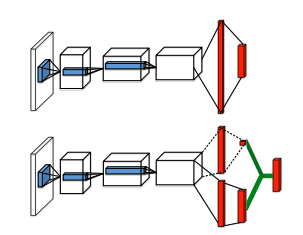
\includegraphics[scale=0.9]{dueling.png}
    \\
    Fig: The Dueling DQN architecture (Image taken from the original paper by Wang et al.)
    \end{center}\\
    
    The q-value in a Dueling DQN architecture is given by 
    \begin{align}
	Q(s_t, a_t) = V(s_t) + A(a)
    \end{align}
    where,\\
    
\hspace*{10mm}V(s\_t) \hspace*{5mm}= \hspace*{5mm}The value of the current state (how advantageous it is to be in that \hspace*{33mm}state)

\hspace*{10mm}A(a) \hspace*{8mm}=\hspace*{5mm}The advantage of taking action an a at that state

\section{About the project}

My original goal for the project was to train an agent using DQN to play \textbf{Airstriker Genesis}, a space shooting game and evaluate the same agent's performance on another similar game called \textbf{Starpilot}. Unfortunately, I was unable to train a decent enough agent in the first game, which made it meaningless to evaluate it's performance on yet another game. 

Because I still want to do the original project some time in the future, to prepare myself for that I thought it would be better to first learn in-depth about how Deep Q-Networks work, what their shortcomings are and how they can be improved. This, and for time-constraint reasons, I have changed my project for this class to a comparison of various DQN versions.


\section{Dataset}
I used the excellent \href{https://github.com/openai/gym}{Gym} library to run my environment. A total of 9 agents, 1 in Airstriker Genesis, 4 in Starpilot and 4 in Lunar Lander were trained. 


\begin{longtable}{|p{2cm}|p{6cm}|p{4cm}|} % centered columns (4 columns)
\hline\hline %inserts double horizontal lines
\textbf{Game} & \textbf{Observation Space} & \textbf{Action Space} \\  % inserts table
%heading
\hline
Airstriker Genesis & RGB values of each pixel of the game screen \newline(255, 255, 3) & Discrete(12) representing each of the buttons on the old Atari controllers. But since only three of those buttons were used in the game\, the action space was reduced to 3 during training.\newline
( Left, Right, Fire )\\
\hline
Starpilot & RGB values of each pixel of the game screen \newline (64, 64, 3)& Discrete(15) representing each of the button combos \newline  ( Left, Right, Up, Down, Up + Right, Up + Left, Down + Right, Down + Left, W, A, S, D, Q, E, Do nothing ) \\
\hline
Lunar Lander & 8-dimensional vector: \newline 
( X-coordinate, Y-coordinate, Linear velocity in X, Linear Velocity in Y, Angle, Angular Velocity, Boolean (Leg 1 in contact with ground), Boolean (Leg 2 in contact with ground) )& Discrete(4)\newline ( Do nothing, Fire left engine, Fire main engine, Fire right engine ) \\
\hline
\end{longtable}

\textbf{Environment/Libraries}: \\

Miniconda, Python 3.9, Gym, Pyorch, Numpy, Tensorboard on my personal Macbook Pro (M1)

\section{ML Methodology}

Each agent was trained using DQN or one of its flavors. Each agent for a particular game was trained with the same hyperparameters with just the underlying algorithm different. The following metrics for each agent were used for evaluation:
\begin{itemize}
    \item \textbf{Epsilon value over each episode} Shows what the exploration rate was at the end of each episode.
    \item \textbf{Average Q-value for the last 100 episodes} A measure of the average q-value (for the action chosen) for the last 100 episodes.
    \item \textbf{Average length for the last 100 episodes} A measure of the average number of steps taken in each episode 
    \item \textbf{Average loss for the last 100 episodes} A measure of loss during learning in the last 100 episodes (A Huber Loss was used)
    \item \textbf{Average reward for the last 100 episodes} A measure of the average reward the agent accumulated over the last 100 episodes
\end{itemize}
\pagebreak

\subsection{Preprocessing}
For the Airstriker and the Starpilot games:
\begin{enumerate}
    \item Changed each frame to grayscale\\
    Since the color shouldn't matter to the agent, I decided to change the RGB image to grayscale
    \item Changed observation space shape from (height, width, channels) to (channels, height, width) to make it compatible with Pytorch\\ Apparently Pytorch uses a different format than the direct output of the gym environment. For this reason, I had to reshape each observation to match Pytorch's scheme (this took me a very long time to figure out, but had an "Aha!" moment when I remember you saying something similar in class).
    \item Framestacking\\
    Instead of processing 1 frame at a time, process 4 frames at a time. This is because just 1 frame is not enough information for the agent to decide what action to take.
\end{enumerate}

For Lunar Lander, since the reward changes are very drastic (sudden +100, -100, +200) rewards, I experimented with Reward Clipping (clipping the rewards to [-1, 1] range) but this didn't seem to make much difference in my agent's performance.

\end{itemize}

\pagebreak
\section{Results}

\begin{itemize}
    \item \textbf{Airstriker Genesis}\\
    The loss went down until about 5200 episodes but after that it stopped going down any further. Consequently the average reward the agent accumulated over the last 100 episodes pretty much plateaued after about 5000 episodes. On analysis, I noticed that my exploration rate at the end of the 7000th episode was still about 0.65, which means that the agent was taking random actions more than half of the time. On hindsight, I feel like I should have trained more, at least until the epsilon value (exploration rate) completely decayed to 5\%.\\ 
    
    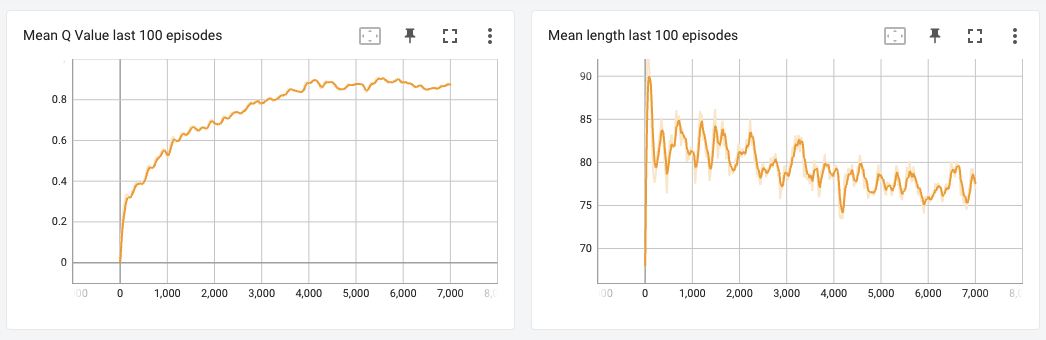
\includegraphics[scale=0.4]{air1.png}
    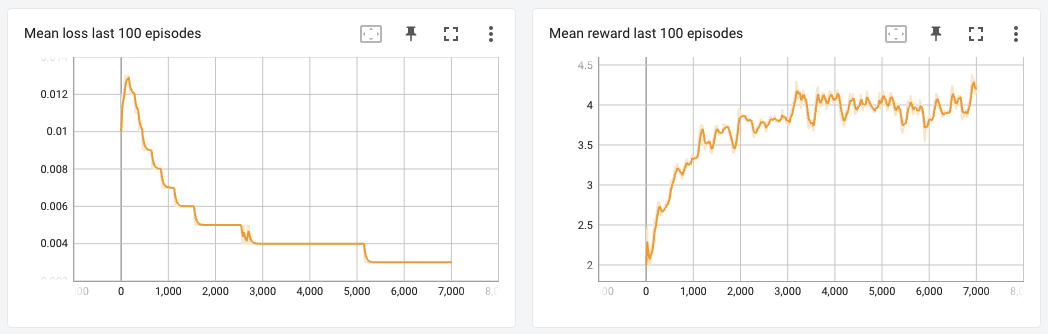
\includegraphics[scale=0.4]{air2.png}
    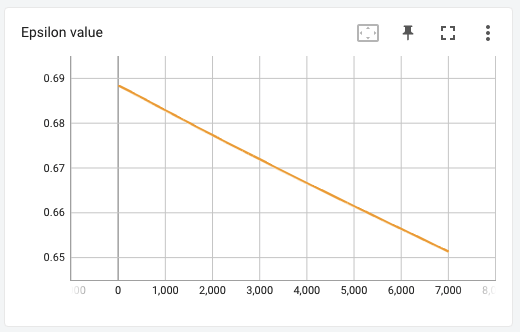
\includegraphics[scale=0.4]{air3.png}\\\\

    \item \textbf{Starpilot}\\\\
    I trained DQN, Double DQN, Dueling DQN and Dueling Double DQN versions for this game to compare the different algorithms.\\
    From the graph of mean q-values, we can tell that the Vanilla DQN versions indeed give high q-values, and their Double-DQN couterparts give lower values, which makes me think that my implementation of the Double DQN algorithm was OK. I had expected the agent to accumulate higher rewards starting much earlier for the Double and Dueling versions, but since the average rewards was almost similar for all the agents, I could not notice any stark differences between the performance of each agent. \\\\
    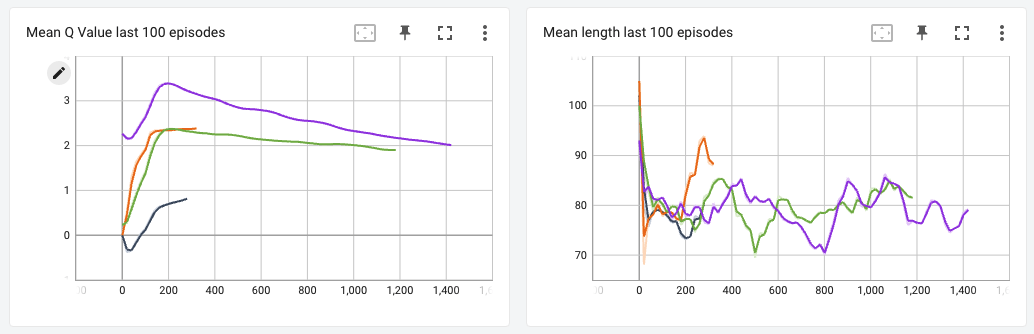
\includegraphics[scale=0.4]{star1.png}\\\\
    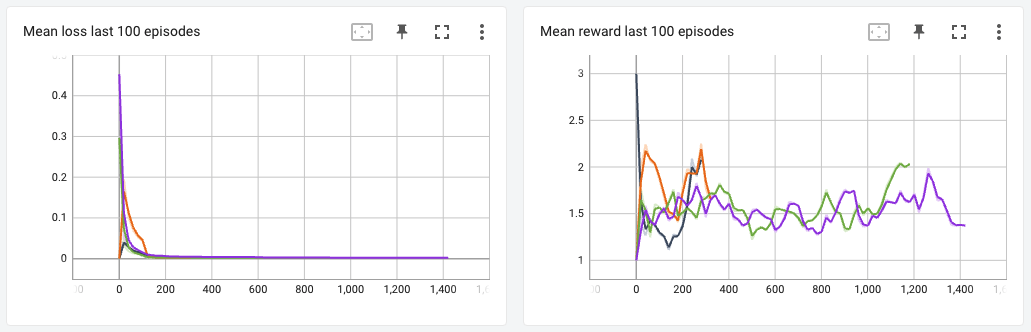
\includegraphics[scale=0.4]{star2.png}
    \begin{figure}[h]
    \begin{tabular}{ll}
    \hspace*{8mm}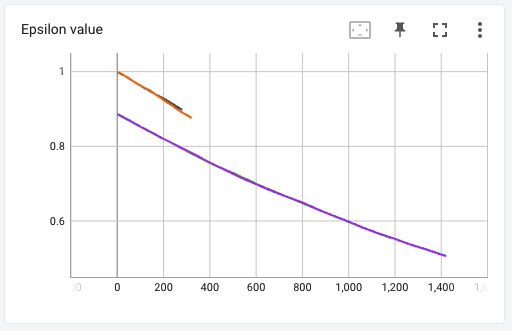
\includegraphics[width=0.5\linewidth]{star3.png}
    &
    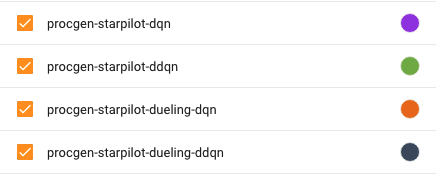
\includegraphics[scale=0.4]{star4.png}
    \end{tabular}
    \end{figure}

    \item \textbf{Lunar Lander}\\\\
    Since I did gain much insight from the agent in the Starpilot game, I thought I was not training long enough. So I tried training the same agents on Lunar Lander, which is a comparatively simpler game with a smaller observation space and one that a DQN algorithm should be able converge pretty quickly to (based on comments by other people in the RL community).\\

    
    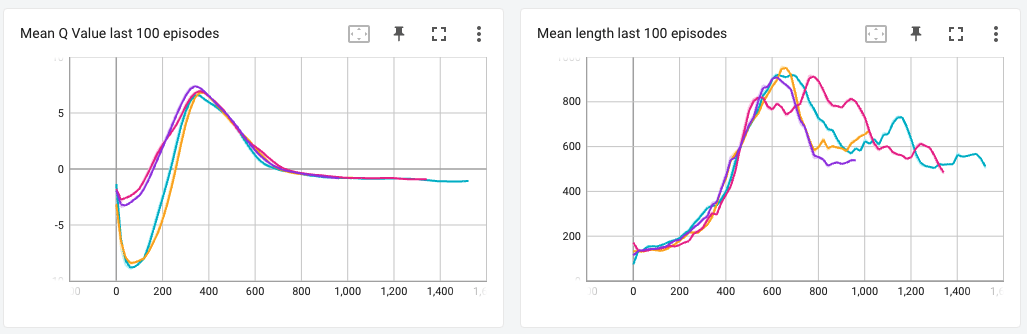
\includegraphics[scale=0.4]{lunar1.png}\\\\
    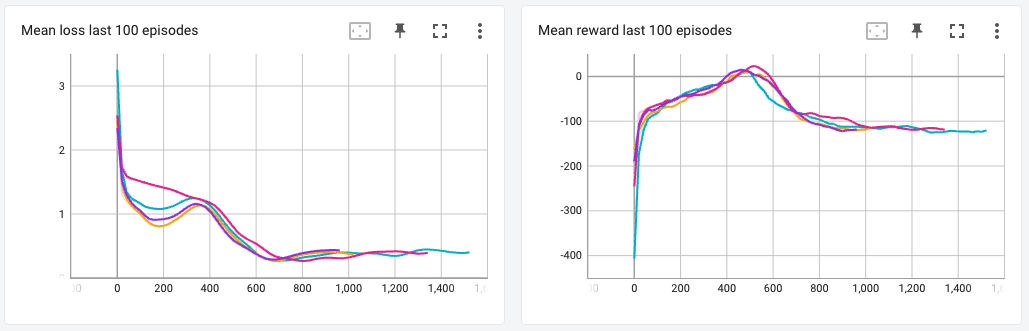
\includegraphics[scale=0.4]{lunar2.png}
    \begin{figure}[h]
    \begin{tabular}{ll}
    \hspace*{8mm}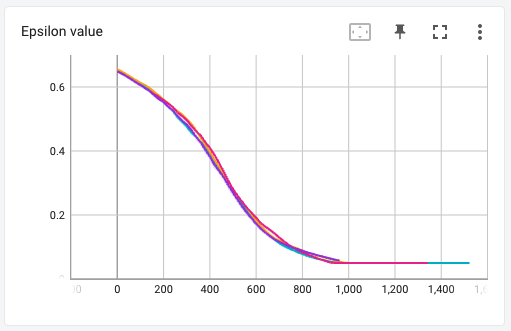
\includegraphics[width=0.5\linewidth]{lunar3.png}
    &
    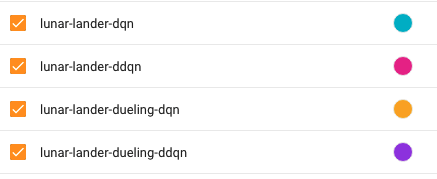
\includegraphics[scale=0.4]{lunar4.png}
    \end{tabular}
    \end{figure}\\
    The results for this were interesting. Although I did not find any vast difference between the different variations of the DQN algorithm, I found that the performance of my agent suddenly got worse at around 300 episodes. Upon researching on why this may have happened, I learned that DQN agents suffer from \textbf{catastrophic forgetting} i.e. after training extensively, the network suddenly forgets what it has learned in the past and the starts performing worse. Initially, I thought this might have been the case, but since I haven't trained long enough, and because all models started performing worse at almost exactly the same episode number, I think this might be a problem with my code or some hyperparameter that I used.

    Upon checking what the agent was doing in the actual game, I found that it was playing it very safe and just constantly hovering in the air, not attempting to land the spaceship (the goal of the agent is to land within the yellow flags). I thought maybe penalizing the rewards for taking too many steps in the episode would work, but that didn't help either.
     \begin{center}
    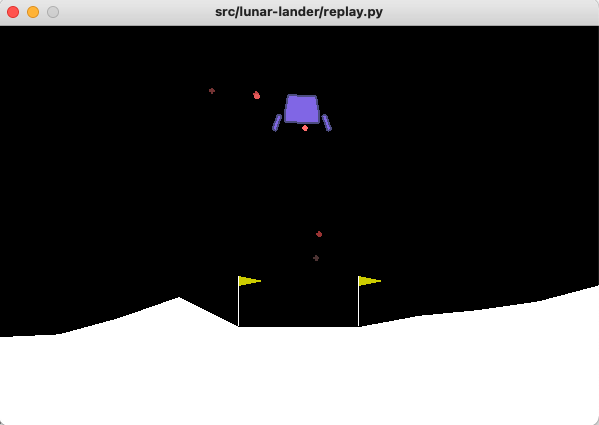
\includegraphics[scale=0.5]{check.png}
    \end{center}
\end{itemize}

\section{Problems Faced}\\
Here are a few of the problems that I faced while training my agents:
\begin{itemize}
    \item Understanding the various hyperparameters in the algorithm. DQN uses a lot of moving parts and thus, tuning each parameter was a difficult task. There were about 8 different hyperparameters (some correlated) that impacted the agent's training performance. I struggled with understanding how each parameter impacted the agent and also with figuring out how to find optimal values for those. I ended up tuning them by trial and error.
    \item I got stuck for a long time figuring out why my convolutional layer was not working. I didn't realize that Pytorch has the channels in the first dimension, and because of that, I was passing huge numbers like 255 (the height of the image) into the input dimension for a Conv2D layer.
    \item I struggled with knowing how long is long enough to realize that a model is not working. I trained a model on Airstriker Genesis for 14 hours just to realize later that I had set a parameter incorrectly and had to retrain all over again.
\end{itemize}

\section{What Next?}
Although I didn't get a final working agent for any of the games I tried, I feel like I have learned a lot about reinforcement learning, especially about Deep Q-learning. I plan to improve upon this further, and hopefully get an agent to go far into at least one of the games. Next time, I will start with first debugging my current code and see if I have any implementation mistakes. Then I will train them a lot longer than I did this time and see if it works. While learning about the different flavors of DQN, I also learned a little about NoisyNet DQN, Rainbow-DQN and Prioritized Experience Replay. I couln't implement these for this project, but I would like to try them out some time soon.

\section{Lessons Learned}

\begin{itemize}
    \item Reinforcement learning is a very challenging problem. It takes a substantially large amount of time to train, it is hard to debug and it is very difficult to tune its hyperparameters just right. It is a lot different from supervised learning in that there are no actual labels and thus, this makes optimization very difficult. 
    \item I tried training an agent on the Atari Airstriker Genesis and the procgen Starpilot game using just the CPU, but this took a very long time. This is understandable because the inputs are images and using a GPU would have been obviously better. Next time, I will definitely try using a GPU to make training faster.
    \item Upon being faced with the problem of my agent not learning, I went into research mode and got to learn a lot about DQN and its improved versions. I am not a master of the algorithms yet (I have yet to get an agent to perform well in the game), but I feel like I understand how each version works. 
    \item Rather than just following someone's tutorial, also reading the actual papers for that particular algorithm helped me understand the algorithm better and code it.
    \item Doing this project reinforced into me that I love the concept of reinforcement learning. It has made me even more interested into exploring the field further and learn more.
\end{itemize}

\pagebreak
\section{References / Resources}
\begin{itemize}
    \item \href{https://pytorch.org/tutorials/intermediate/reinforcement_q_learning.html}{Reinforcement Learning (DQN) Tutorial, Adam Paszke}
    \item \href{https://pytorch.org/tutorials/intermediate/mario_rl_tutorial.html}{Train a mario-playing RL agent, Yuansong Feng, Suraj Subramanian, Howard Wang, Steven Guo}
    \item \href{https://horomary.hatenablog.com/entry/2021/02/06/013412}{About Double DQN, Dueling DQN}
    \item \href{https://arxiv.org/abs/1511.06581}{Dueling Network Architecture for Deep Reinforcement Learning (Wang et al., 2015))}\\\\\\
    \emph{(Final source code for the project can be found} \href{https://github.com/00ber/ml-reinforcement-learning}{\emph{here}}\emph{)}.
\end{itemize}




%%% End document
\end{document}